\chapter{\texorpdfstring{$2d/4d$ correspondance}{2d4d}}
This theory is relevant for the $2d-4d$ correspondence where a $6d$ theory is put on a product space $X_4\times C_2$ 
\begin{equation}
	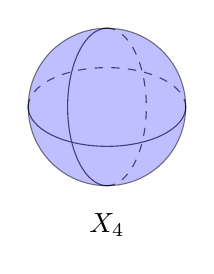
\begin{tikzpicture}[baseline={(0,0)}]
		\draw (-1,0) arc (180:360:1cm and 0.5cm);
    	\draw[dashed] (-1,0) arc (180:0:1cm and 0.5cm);
    	\draw (0,1) arc (90:270:0.5cm and 1cm);
    	\draw[dashed] (0,1) arc (90:-90:0.5cm and 1cm);
 		\filldraw[fill=blue!50, opacity=.5] (0,0) circle (1cm);

		\node at (0,-1.5) {$X_4$};
	\end{tikzpicture}\qquad\times\qquad
	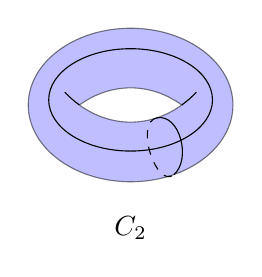
\begin{tikzpicture}[scale=1.3, baseline={(0,0)}]
		\draw[fill=blue!50,opacity=.5,even odd rule] (0,0) ellipse (1 and .75) 
		(-0.5,0) arc(120:60:1 and 1.25)  arc(-60:-120:1 and 1.25) coordinate[pos=0.25] (xt);
	   \draw (-0.5,0) arc(-120:-130:1 and 1.25) (0.5,0) arc(-60:-50:1 and 1.25);
	   \draw[] (-65:1 and .75) to[out=40,in=10] 
		node[pos=0.2,right]{} (xt);
	   \draw[dashed] (xt) to[out=-170,in=-140] (-65:1 and .75);
	   \draw[] (0.8,0.05) arc(0:360:0.8 and .5) {};
	   \node at (0,-1.2) {$C_2$};
	\end{tikzpicture}
\end{equation}
and compactified either on the first factor or on the second one. In the partition function of the $6d$ theory is a nice SUSY partition function that does not depende on the sizes of the two factors, then we expect the lower dimentional partition functions to match. Pictorially
\begin{equation*}
\begin{array}{rcl}
	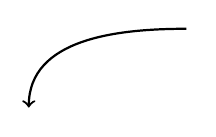
\begin{tikzpicture}[baseline={(0,0)}]
		\draw[->, thick] (0,0) to [out=180, in=90] (-2,-1);
	\end{tikzpicture}
	&\cZ_{S_{6d}}\left(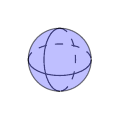
\begin{tikzpicture}[scale=.4,baseline={(0,-.1)}]
		\draw (-1,0) arc (180:360:1cm and 0.5cm);
    	\draw[dashed] (-1,0) arc (180:0:1cm and 0.5cm);
    	\draw (0,1) arc (90:270:0.5cm and 1cm);
    	\draw[dashed] (0,1) arc (90:-90:0.5cm and 1cm);
 		\filldraw[fill=blue!50, opacity=.5] (0,0) circle (1cm);
	\end{tikzpicture}\times
	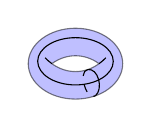
\begin{tikzpicture}[scale=.6, baseline={(0,-.1)}]
		\draw[fill=blue!50,opacity=.5,even odd rule] (0,0) ellipse (1 and .75) 
		(-0.5,0) arc(120:60:1 and 1.25)  arc(-60:-120:1 and 1.25) coordinate[pos=0.25] (xt);
	   \draw (-0.5,0) arc(-120:-130:1 and 1.25) (0.5,0) arc(-60:-50:1 and 1.25);
	   \draw[] (-65:1 and .75) to[out=40,in=10] 
		node[pos=0.2,right]{} (xt);
	   \draw[dashed] (xt) to[out=-170,in=-140] (-65:1 and .75);
	   \draw[] (0.8,0.05) arc(0:360:0.8 and .5) {};
	\end{tikzpicture}\right)&
	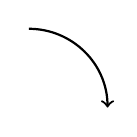
\begin{tikzpicture}[baseline={(0,0)}]
		\draw[thick, ->] (0,0) to [out=0, in=90] (1,-1);
	\end{tikzpicture}\\[15pt]
	%%%%%%%%%%%%%%%%%%%%%%%%%%%%%
	%%%%%%%%%%%%%%%%%%%%%%%%%%%%%
	\cZ_{S_{2d}\left[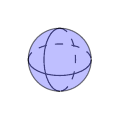
\begin{tikzpicture}[scale=.4,baseline={(0,0)}]
		\draw (-1,0) arc (180:360:1cm and 0.5cm);
		\draw[dashed] (-1,0) arc (180:0:1cm and 0.5cm);
		\draw (0,1) arc (90:270:0.5cm and 1cm);
		\draw[dashed] (0,1) arc (90:-90:0.5cm and 1cm);
		\filldraw[fill=blue!50, opacity=.5] (0,0) circle (1cm);
	\end{tikzpicture}\right]}\left(
	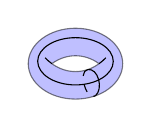
\begin{tikzpicture}[scale=.6, baseline={(0,0)}]
		\draw[fill=blue!50,opacity=.5,even odd rule] (0,0) ellipse (1 and .75) 
		(-0.5,0) arc(120:60:1 and 1.25)  arc(-60:-120:1 and 1.25) coordinate[pos=0.25] (xt);
		\draw (-0.5,0) arc(-120:-130:1 and 1.25) (0.5,0) arc(-60:-50:1 and 1.25);
		\draw[] (-65:1 and .75) to[out=40,in=10] 
		node[pos=0.2,right]{} (xt);
		\draw[dashed] (xt) to[out=-170,in=-140] (-65:1 and .75);
		\draw[] (0.8,0.05) arc(0:360:0.8 and .5) {};
	\end{tikzpicture}\right)
	&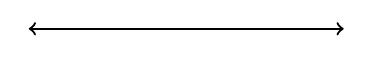
\begin{tikzpicture}[baseline={(0,0)}]
		\draw[thick,<->] (1,0) -- (5,0);
	\end{tikzpicture}&\cZ_{S_{4d}\left[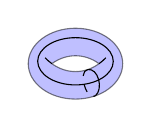
\begin{tikzpicture}[scale=.6, baseline={(0,0)}]
		\draw[fill=blue!50,opacity=.5,even odd rule] (0,0) ellipse (1 and .75) 
		(-0.5,0) arc(120:60:1 and 1.25)  arc(-60:-120:1 and 1.25) coordinate[pos=0.25] (xt);
		\draw (-0.5,0) arc(-120:-130:1 and 1.25) (0.5,0) arc(-60:-50:1 and 1.25);
		\draw[] (-65:1 and .75) to[out=40,in=10] 
		node[pos=0.2,right]{} (xt);
		\draw[dashed] (xt) to[out=-170,in=-140] (-65:1 and .75);
		\draw[] (0.8,0.05) arc(0:360:0.8 and .5) {};
	\end{tikzpicture}\right]}\left(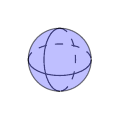
\begin{tikzpicture}[scale=.4,baseline={(0,0)}]
		\draw (-1,0) arc (180:360:1cm and 0.5cm);
		\draw[dashed] (-1,0) arc (180:0:1cm and 0.5cm);
		\draw (0,1) arc (90:270:0.5cm and 1cm);
		\draw[dashed] (0,1) arc (90:-90:0.5cm and 1cm);
		\filldraw[fill=blue!50, opacity=.5] (0,0) circle (1cm);
	\end{tikzpicture}\right)
\end{array}
\end{equation*}
These lower dimensional theories have been studied and loosely follow this classification
\begin{itemize}
	\item
		$S_{4d}\left[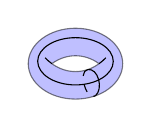
\begin{tikzpicture}[scale=.6, baseline={(0,-.1)}]
			\draw[fill=blue!50,opacity=.5,even odd rule] (0,0) ellipse (1 and .75) 
			(-0.5,0) arc(120:60:1 and 1.25)  arc(-60:-120:1 and 1.25) coordinate[pos=0.25] (xt);
			\draw (-0.5,0) arc(-120:-130:1 and 1.25) (0.5,0) arc(-60:-50:1 and 1.25);
			\draw[] (-65:1 and .75) to[out=40,in=10] 
			node[pos=0.2,right]{} (xt);
			\draw[dashed] (xt) to[out=-170,in=-140] (-65:1 and .75);
			\draw[] (0.8,0.05) arc(0:360:0.8 and .5) {};
		\end{tikzpicture}\right]$ : where $C_2$ is any Riemann surface with, possibly, punctures, are known class-S theories
	\item $S_{2d}\left[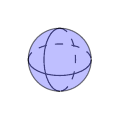
\begin{tikzpicture}[scale=.4,baseline={(0,-.1)}]
		\draw (-1,0) arc (180:360:1cm and 0.5cm);
		\draw[dashed] (-1,0) arc (180:0:1cm and 0.5cm);
		\draw (0,1) arc (90:270:0.5cm and 1cm);
		\draw[dashed] (0,1) arc (90:-90:0.5cm and 1cm);
		\filldraw[fill=blue!50, opacity=.5] (0,0) circle (1cm);
	\end{tikzpicture}\right]$: where $X_4=S^4$ is known as $2d$ Liouville-Toda theory
	\item $S_{2d}\left[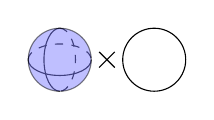
\begin{tikzpicture}[scale=.4,baseline={(0,-.1)}]
		\draw (-1,0) arc (180:360:1cm and 0.5cm);
		\draw[dashed] (-1,0) arc (180:0:1cm and 0.5cm);
		\draw (0,1) arc (90:270:0.5cm and 1cm);
		\draw[dashed] (0,1) arc (90:-90:0.5cm and 1cm);
		\filldraw[fill=blue!50, opacity=.5] (0,0) circle (1cm);
		\draw plot[mark=x,scale=5] coordinates{(0.30,0)};
		\draw (3,0) circle (1cm);
	\end{tikzpicture}\right]$: where $X_4=S^3\times S^1$ is known as $2d$ $q$-deformed YM
\end{itemize}
\section{\texorpdfstring{$2d$ Yang-Mills}{2dYM}}
In $2d$ there is no physical propagating degrees of freedom. Take $G$ to be a non-abelian Lie group. The action is of the form
\begin{equation}
	S\propto=\frac{1}{e^2}\int \dd[2]{x}\sqrt{\det g}\Tr F^2
\end{equation}
In $2d$ the only non-zero component of the curvature tensor is $F_{01}$ therefore
\begin{equation}
	\Tr F_{\mu\nu}F^{\mu\nu}=(g^{00}g^{11}-g^{01}g^{10})\Tr F_{01}^2=\det g^{-1}\Tr F_{01}^2
\end{equation}
so that 
\begin{equation}
	S \propto\frac{1}{e^2}\int\dd[2]{x}\sqrt{\det g}^{-1}\Tr F_{01}^2
\end{equation}
Therefore, the action only depends on the area of the surface, there is no additional dependence on the metric. This is a very special kind of $2d$ QFT. Whenever such a QFT is also a CFT, the theory is a $2d$ TQFT. The dependence on the coupling can be reabsorbed in the definition of the area.

We can solve this theory in many ways, but let us consider the Hamiltonian formalism putting the theory on cylinder. 
\begin{equation}
	\begin{tikzpicture}[transform shape]
		\pic[
			tqft/cylinder, 
			rotate=90,
			fill=blue!50,
			scale=2,
			opacity=.5,
			cobordism edge/.style={draw},
			incoming upper boundary component 1/.style={draw, fill=red!50, opacity=.5},
			incoming lower boundary component 1/.style={draw, fill=red!50, opacity=.5},
			outgoing lower boundary component 1/.style={draw, dashed},
			outgoing upper boundary component 1/.style={draw},
			view from=incoming,
			at={(0,0)},
			every node/.style={transform shape},
			name=a
		];
		\draw[overlay,
				shift=(a-outgoing boundary), 
				xscale=.5,
				decoration={markings, mark=at position 0.8 with {\arrow{>}}}, 
				postaction={decorate}] {(1.5,0)} circle (.7) node[above left,yshift= 10pt, xshift=-15pt, thick] {};
		\draw[<->, thick, transform canvas={yshift=-1cm}] (a-incoming boundary.north) --node[below] {$T$}  (a-outgoing boundary.south) ;
		\node (L) at (5.3,0.7) {$L$};
		\draw[->, thick, transform canvas={xshift=.3cm,yshift=.2cm}] (a-incoming boundary) to [out=180,in=90] (-2,-1) node[below] {$\cH_{S^1}$};
	\end{tikzpicture}
\end{equation}\\

On $S^1$ we have an Hilbert space of states which, by taking the length of the circle to be $L$ can be defined as follows
\begin{equation}
	G\ni U=\text{Pexp}\int_0^L A_1 \dd x^1
\end{equation}
which is almost gauge invariant. At $0$ we still have a residual gauge transformation
\begin{equation}
	U\to gUg^-1
\end{equation}
So the Hilbert space is spanned by wavefunctions of $U$ which are invariant under the residual gauge transformation 
\begin{equation}
	\cH_{S^1}\ni \Psi(U)=\Psi(gUG^-1)
\end{equation}
One such basis for this Hilbert space is given by the characters of the representation $\chi_R(U)=\Tr_R U$ (class functions) which are indeed invariant under adjoint action. Moreover these are orthogonal given the following inner product
\begin{equation}
	\int \chi_R(U)\overline{\chi_{R^\prime}(U)}\dd{[U]}_{\text{Haar}}=\delta_{RR^\prime}
\end{equation}
Using the standard canonical quantization procedure, we can also find the Hamiltonian of the system. Being the only non-zero component of the curvature $F_{01}=E$, we have no magnetic field and therefore 
\begin{equation}
	H=\int_0^L\abs{E}^2\dd{x^1}=\int_0^L\frac{\delta}{\delta A_1(x_1)}\frac{\delta}{\delta A_1(x_1)}
\end{equation}
The action of the Hamiltonian on the basis is easily computed
\begin{equation}
\begin{split}
	H \chi_R(U) &= H \Tr_R\text{Pexp}\int_0^L T^a A_1^a\dd{x^1}\\
	&=\Tr_R\qty(\int_0^L T^a T^a) \dd{x^1}\Tr_R\text{Pexp}\int_0^L T^a A_1^a\dd{x^1}\\
	&=L c_2(R) \chi_R(U)
\end{split}
\end{equation}
which proves that the characters are indeed eigenstates of the hamiltonian. We can further idenfity the sides of the cylinder to get a torus $\bbT^2=S^1\times S^1$ and compute the partition function 
\begin{equation}
	Z_{2d}=\Tr_{\cH_{S^1}}e^{-HT}=\sum_R e^{-TL c_2(R)}
\end{equation}
which only depends on the area $TL$.

Next step, let us consider the following geometry: a disk with area $A$ (a cigar) 
\begin{equation}
	\begin{tikzpicture}[transform shape]
		\pic[
			tqft/cap,
			rotate=-90,
			scale=2,
			fill=blue!50,
			opacity=.5,
			cobordism edge/.style={draw},
			every outgoing boundary component/.style={draw},
			name=a
		];
		\draw[->, thick] (-3.3,0) -- (-2,0) node[right] {$A$};
		\draw[->, thick, transform canvas={yshift=-.6cm, xshift=-.4cm}] (a-outgoing boundary) to[in=90,out=90] (-5,-.4) node[below] {$\cH_{S^1}\ni\Psi_A(U)$};
	\end{tikzpicture}
\end{equation}\\
where now
\begin{equation}
	\cH_{S^1}\ni \Psi_A(U)
\end{equation}
which we like to determine (Hartle-Hawking wavefunction). To determine it we can consider joining a cylinder with area $A^\prime$ to the cigar and get\\

\begin{minipage}[c]{0.4\textwidth}
	\centering
		\begin{tikzpicture}[baseline={(0,-.2)}, transform shape]
			\pic[
				tqft/cap,
				scale=1.5,
				fill=blue!50,
				opacity=.5,
				cobordism edge/.style={draw},
				every outgoing boundary component/.style={fill=blue!50},
				name=h,
				rotate=90
			];
			\pic[
				tqft/cylinder, 
				fill=blue!50,
				scale=1.5,
				at=(h-outgoing boundary 1),
				opacity=.5,
				cobordism edge/.style={draw},
				incoming upper boundary component 1/.style={draw},
				incoming lower boundary component 1/.style={draw, dashed},
				outgoing lower boundary component 1/.style={draw, dashed},
				outgoing upper boundary component 1/.style={draw},
				view from=incoming,
				name=a,
				rotate=90
			];
		\end{tikzpicture}
	\end{minipage}
\begin{minipage}[c]{0.55\textwidth}
\begin{equation}
	\Psi_{A+A^\prime}(U)=e^{-A^\prime H}\Psi_A(U)
\end{equation}
\end{minipage}\\[10pt]
since we can easily change the area it is sufficient to know the zero area wavefunction. This can be understood from a path integral point of view. We have our spacetime to which there is cut out a zero-area disk. The holonomy around it needs to be one. Therefore the zero-area limit of this wavefunction must be a delta function. This is not square-integrable but we just add a constant
\begin{equation}
	\Psi_A(U)=\alpha\delta(U)=\sum_R f_R\chi_R(U)
\end{equation}
where the constants can be found as
\begin{equation}
	\alpha\chi_{R^\prime}(1)=f_{R^\prime}
\end{equation}
so that $f_R=\alpha \dim R$. Let us consider the pair of pants geometry with area $A$ so that we have three Hilbert spaces which should determine a vector in 
\begin{equation}
	\bigotimes_{i=1,2,3} H_{S^1}\ni \Psi_A(U_1,U_2,U_3)
\end{equation}
depending on the three holonomies.

By gluing a disk to one of the $S^1$ we get a cylinder with area $A+A^\prime$ to which we know the wavefunction. Therefore 
\begin{equation}
	\Psi_A(U_1,U_2,U_3)=\sum_R e^{-A c_2(R)}\frac{\chi_R(U_1)\chi_R(U_2)\chi_R(U_3)}{\dim R}
\end{equation}
We can now glue the three-punctured spheres in various ways to get many different geometries with different genus. For example, for genus $g=1$ with three punctures $n=3$ we can find 
\begin{equation}
	\frac{1}{\alpha^{2g-2+n}}\sum_R e^{-A c_2(R)}\frac{\prod_i \chi_R(U_i)}{(\dim R)^{2g-2+n}}
\end{equation}
Originally the constant $alpha$ came from the fact that the zero-area disk amplitude is a delta function which has to be normalized. On a genus $g$ surface, doing a QFT is very easy to generate a counterterm of the form 
\begin{equation}
	\delta S=\beta\int \dd[2]{x}\sqrt{g}R=\beta (2-2g)
\end{equation}
on a closed Riemann surface. This multiplies $Z$ by 
\begin{equation}
	e^{\beta(2-2g)}
\end{equation}
and the boundaries give some similar quantities depending on $n$. 

\section{$q$-deformed YM}
We consider the gauge group $G$ to be a standard Lie group. We deform it to a quantum group $G_q$ (the matrix entries become non-commutative). Take for example $\SU(2)_q$
\begin{equation}
	\begin{pmatrix}
		\alpha&\beta\\
		-\beta^*&\alpha^*
	\end{pmatrix},\qquad \alpha\beta=q\;\beta\alpha,\; \alpha\beta^*=q\;\beta^*\alpha,\ldots
\end{equation}
So we try to define a $2d$ YM in a lattice formulation for example, where all the link variables are replaced by a quantum group element instead of Lie group elements. This can be done in any dimensions but because of the non-commutativity one needs to define exacly in which order each link variable appears in the path integral. This is known at least in two dimensions how to do it consistently. In general dimensions is not known\dots

The end result is simple actually. Just replice the dimension of the rep by it's quantum dimension. When $G=\SU(N)_q$, then 
\begin{equation}
	\dim_q R = \chi_R\qty(\text{diag}(q^{\frac{N-1}{2}},q^{\frac{N-3}{2}},\cdots,q^{\frac{1-N}{2}})) 
\end{equation}
which in the limit $q\rightarrow1$ becomes $\chi_R(1)=\dim R$ as expected.

\section{Relation between Gaiotto theories and $q$-deformed YM}
Consider the superconformal index of $\cN=2$ $\SU(2)$ with $N_f=4$ flavours. This theory enjoys a special kind of S-duality discussed before. 

The relevant step in recongnizing the relationship between this theory and the $q$-deformed YM theory, is to consider the SCI of the Gaiotto theory in the limit of $q=t$. Consider in fact the half hypermultiplet contribution to the index 
\begin{equation}
	\Gamma(t^{1/2}z^\pm a^\pm b^\pm;p,q)\Gamma(t^{1/2}z^\pm c^\pm d^\pm;p,q)
\end{equation}
which explicitly, with $q=t$, gives
\begin{equation}
	\Gamma(t^{1/2}z^\pm;p,q)=\prod_{m,n\ge 0}\frac{1-z^{-1}p^{m+1}q^{n+\frac{1}{2}}}{1-zp^m q^{n+\frac{1}{2}}}\frac{1-z p^{m+1}q^{n+\frac{1}{2}}}{1-z^{-1}p^m q^{n+\frac{1}{2}}}
\end{equation}
There is a quasi complete cancellation between numerator and denominator such that the whole product just becomes
\begin{equation}
	\prod_{n\ge0}\frac{1}{1-q^{n+\frac{1}{2}}z}\frac{1}{1-q^{n+\frac{1}{2}}z^{-1}}
\end{equation}
and the dependence on $p$ vanished (this is a general behavior for $\cN=2$ SCFTs). This is due to the enanchement of SUSY in the aformentioned limit. 

So for the SCI of the original Gaiotto theory becomes 
\begin{equation}
	\frac{1}{2}\oint \frac{\dd z}{2\pi \I z}(1-z^2)(1-z^{-2})K(z)^{-2}\prod_{\pm\pm\pm}\prod_{n\ge 0}\frac{1}{1-q^{n+\frac{1}{2}}z^\pm a^\pm b^\pm}\frac{1}{1-q^{n+\frac{1}{2}}z^\pm c^\pm d^\pm}
\end{equation}
where
\begin{equation}
	K(z)^{-1}=\prod_{n\ge 0}(1-q^{n+1})\prod_\pm (1-q^{n+1}z^{\pm 2})
\end{equation}
The matter contribution can be rewritten with an infinite sum insted of an infinite product
\begin{equation}
	\prod_{\pm\pm\pm}\prod_{n\ge0}\frac{1}{1-q^{+\frac{1}{2}}z^\pm a^\pm b^\pm}=\frac{K(z)K(a)K(b)}{K_0}\sum_{n\ge 1}\frac{\chi_n(z)\chi_n(a)\chi_n(b)}{\chi_n(q^{\frac{1}{2}})}
\end{equation}
where
\begin{equation}
	\chi_n(a)=a^{n-1}+a^{n-3}+\cdots+a^{1-n}
\end{equation}
which is the character of 
\begin{equation}
	\begin{pmatrix}
		a&0\\
		0&a^{-1}
	\end{pmatrix}\in \SU(2)
\end{equation}
in the $n$-dimensional rep of $\SU(2)$, and
\begin{equation}
	K_0^{-1}=\prod_{n\ge0}(1-q^{2+n})
\end{equation}

We can plug this in the SCI formula and find
\begin{equation}
	\begin{split}
	\frac{1}{2}\oint &\frac{\dd{z}}{2\pi \I z}(1-z^2)(1-z^{-2})K(z)^{-2}\frac{K(z)K(a)K(b)}{K_0}\sum_{n\ge 1}\frac{\chi_n(z)\chi_n(a)\chi_n(b)}{\chi_n(q^{\frac{1}{2}})}\\
	&\times\frac{K(z)K(c)K(d)}{K_0}\sum_{m\ge 1}\frac{\chi_m(z)\chi_m(c)\chi_m(d)}{\chi_m(q^{\frac{1}{2}})}
	\end{split}
\end{equation}
The dependence on $z$ is localized now. Now $K(z)$ cancels out and the only $z$ dependent factors are in the charachers. There is a formula 
\begin{equation}
	\frac{1}{2}\oint \frac{\dd{z}}{2\pi \I z}(1-z^2)(1-z^{-2})\chi_m(z)\chi_n(z)=\delta_{m,n}
\end{equation}
since this is the orthogonal condition of the character on the torus of $\SU(2)$. Therefore the final result simplyfies a lot
\begin{equation}
	\frac{K(a)K(b)K(c)K(d)}{K_0^2}\sum_{n\ge 1}\frac{\chi_n(a)\chi_n(b)\chi_n(c)\chi_n(d)}{\chi_n(q^{\frac{1}{2}})^2}
\end{equation}
And now the invariance under the exchange of the various letters is manifest! But this is also just the partition function of $q$-deformed YM on a four punctured sphere with holonomies $a,b,c,d$ with the area sent to zero\\[10pt]
\begin{minipage}[c]{0.5\textwidth}
\centering
	\begin{tikzpicture}[baseline={(0,0)}]
		\pic[
			tqft,
			incoming boundary components=2,
			outgoing boundary components=2,
			offset =0,
			fill =blue!50 ,
			opacity=.5,
			cobordism edge/.style={draw} ,
			incoming upper boundary component 1/.style={draw},
			incoming upper boundary component 2/.style={draw},
			incoming lower boundary component 1/.style={draw, dashed},
			incoming lower boundary component 2/.style={draw, dashed},
			every outgoing boundary component/.style={draw},
			name=a
			];
			\foreach \anchor/\x/\name/\shift in {incoming boundary 1/above left/a/+, incoming boundary 2/above right/b/+, outgoing boundary 1/below left/c/-, outgoing boundary 2/below right/d/-}
			\draw[overlay,
				shift=(a-\anchor), 
				yscale=.5,
				decoration={markings, mark=at position 0.8 with {\arrow{>}}}, 
				postaction={decorate}] {(0,0)} circle (.5) node[\x,yshift=\shift 1.5ex] {$\name$};
			\path (a-incoming boundary) +(0,.5) (a-outgoing boundary) +(0,-1);
	\end{tikzpicture}
\end{minipage}\hspace{-2cm}
\begin{minipage}[c]{0.5\textwidth}
	\begin{equation}
		\xlongrightarrow{A\rightarrow 0} \sum_R\frac{\chi_R(a)\chi_R(b)\chi_R(c)\chi_R(d)}{(\dim_q R)^2}\hspace{2cm}
	\end{equation}
\end{minipage}\\
This is the explicit $4d-2d$ correspondance! 

\section{\texorpdfstring{Connection to $6d$}{Mtheory}}
But why is this the case? The general idea is that each half-hypermultiplet corresponds to a three-punctured sphere and the gauge field is just a tube connecting punctures. 

The fact is that there is a certain $6d$ $\cN=(2,0)$ SCFT labelled by $G=ADE$\footnote{$A_n=\SU(n+1),D_n=\SO(2n),E_n=E_6,E_7,E_8$} such that its compactification on $S^1$ in the IR is given by a $5d$ $\cN=2$ SYM with gauge group $G$. By compactifying the $A_n$ case on the right punctured geometry the $4d$ theory is just the one studyied up to now.

But how do we know this? Starting from string theory, consider $N$ M5-branes on top of each other. The worldsheet theory is just the $6d$ $\cN=(2,0)$ gauge theory with gauge group $A_{N-1}$. For $D_N,E_N$ one can do similar constructions.

Before going to $4d$ $\cN=2$, we want to study $4d$ $\cN=4$ coming from a similar setup. Take the $6d$ SCFT and put it on $S^1$ with a radious $R_6$. The compactified theory is just $5d$ $cN=2$ SYM with $G$ gauge group 
\begin{equation}
	\int \dd[5]{x}\frac{1}{g^2_5}\tr F\wedge\star F+\cdots
\end{equation}
In $5d$ the inverse of the gauge coupling has dimension one since the kinetic term has dimension four. But the SCFT does not have any mass scale, therefore
\begin{equation}
	g_5^2\propto R_6
\end{equation}
Let us do another compactification on a circle with radius $R_5$. This becomes $4d$ $\cN=4$ SYM with gauge group G whose coupling constant is given by a usual Kaluza-Klein expansion
\begin{equation}
	\int \dd x_5\int\dd[4]x\frac{1}{g_5^2}\tr F\wedge \star F+\cdots
\end{equation}
where now the combination of $g_5^{-2}\dd{x_5}=g_{4}^{-2}$ and therefore 
\begin{equation}
	\frac{1}{g_4^2}\sim\frac{R_5}{R_6}
\end{equation}
Here we just put the $6d$ theory on a $T^2$ with sizes $R_6,R_5$ and got a $4d$ theory with $\tau=R_5 /R_6$. We could compactify in the other direction and get another $4d$ $\cN=4$ SYM with $\tau=R_6 / R_5$ which is just the inverse of the other one. This is the S-duality action which in this language is just Lorentz invariance in $6d$. 

In the $4d$ theory, basic excitations are point-like, but in $6d$ we have strings which can wrap the two cycles of the torus. These are tensionful strings, and therefore are massive excitations in the low energy theory. These have masses proportional to their tension and the radius of the two circles. The ratio of the mass of the excitations is just the complexified coupling. Recall that in $\cN=4$ the ratio of the mass of the W-boson and the monopole is given by the coupling $\tau$, so we can identify them with the wrapped strings. They come from the same object in $6d$. If one can write the lagrangian for this theory, S-duality would be completely trivial. But there perturbative excitations are going to be the same as semiclassical ones. This is very difficult.

\subsection{Kaluza-Klein reduction}
Consider a free massless scalar $\phi$ in $d$-dimensions and put it on $S^1$ of radius $R$. We can decompose the field in terms of the Fourier modes
\begin{equation}
	\phi(\vec{x},x_d)=\sum_n\phi_{(n)}(\vec{x})e^{in x_\frac{d}{R}}
\end{equation}
and the excitations are going to have massess of order 
\begin{equation}
	m=\abs{\frac{n}{R}}\quad\text{Kaluza-Klein tower}
\end{equation}
Consider $5d$ $\cN=2$ SYM with gauge group $G$ on flat space $\bbR^4\times \bbR$. This has instanton configurations which is point-like in $\bbR^4$ but it extends in time. It's a particle like excitation and the mass is given by the instanton action: if instanton number is $n$, the mass is 
\begin{equation}
	\frac{8\pi^2}{g_5^2}n\propto \frac{n}{R_6}
\end{equation}
So the mass of the instanton particle behave exactly like the KK tower. They are exactly the same when we fix the proportionality constant as
\begin{equation}
	g_{5d}^2=8\pi R_5^2
\end{equation}
So when we start from $6d$ part of the tower is included by the instanton configurations. There is an empirical fact: as far as BPS quantities are concerned, $5d$ SYM computations including instantons gives all the expected KK modes. In particular, if you add, say, KK towers of $5d$ YM fields, one gets double counting.

So if a lagrangian for this theory, it should have a gigantic gauge symmetry which would gauge away all this KK modes and identify them with the instantons. 

\subsection{Back to $6d$}
Now we can go to the $4d$ $\cN=2$ case. Take $6d$ $\cN=(2,0)$ of type $A_1=\SU(2)$\footnote{This does not mean that there is a $\SU(2)$ gauge field in $6d$.} and put it on a Riemann surface made of two $3$-punctured spheres glues on one puncture. Let us say that the tube has circumference length $R_6$ and length $R_5$. Use the fact that when we compactify the theory on a cicle, we get $5d$ $\cN=2$ SYM on a segment coupled to something at the ends. By compactifying again we get a $4d$ gauge multiplet with $\tau=R_5 / R_6$. But there is something going on on the ends, let us say there is a way to have a remaining $\cN=2$ instead of $\cN=4$ due to the boundary conditions. What is this boundary condition? From the $6d$ point of view we cannot say i for sure. But in $5d$ we see that the boundary is $\bbR^4$ so one can have some $4d$ theory with $\SU(2)$ flavour symmetry living on the boundary that couples to the bulk.The theory is exactly the trifundamental hypermultiplet $Q_{ABg}$. So let us try to determine what this $3$-punctured sphere is from $6d$: consider the SCI of the $4d$ theory obtained from $6d$ by putting the theory on this Riemann surface. Morally, the partition function of the $4d$ theory on $S^3\times S^1$ is just the partition function of the $6d$ theory on $S^3\times S^1\times \Sigma_g$. But since there is an $S^1$ we can compactify on it and get the partition function of the $5d$ SYM on $S^3\times \Sigma_g$. When compactifying again on $S^3$, computing the various corrections and including the KK modes around $S^3$ we get the partition function of a $2d$ theory on $\Sigma_g$ which is just $q$-deformed YM.

S-duality can be derived in a very nice way from $6d$. We found that the $6d$ theory on $\Sigma_4$ comprised of two $3$-punctured spheres connected by a cyclinder of circumference $R_6$ and length $R_5 $ gives rise to a $4d$ theory of two trifundamental hypermultiplet and an $\cN=2$ vector multiplet with coupling $\tau= R_5 / R_6$. We can make the coupling very small by having a very long cylinder. When we make the cylinder vert short, the theory is vert strongly coupled and when the two spheres are very near to each other we can split the $2d$ surgface in another way and consider the dimensional reduction along the other direction which just gives the S-dual theory.

\section{\texorpdfstring{Generalizing to $\SU(N)$}{SUN}}
We saw before that by compactifying $6d$ $\cN=(2,0)$ of type $A_1$ on a $3$-punctured sphere we obtain the theory of a free hypermultiplet. This is also confirmed by the structure of the SCI which was discussed and can be found from $6d$. The SCI is just given by 
\begin{equation}
	\frac{K(a)K(b)K(c)K(d)}{K_0^2}\sum_{n\ge 1}\frac{\chi_n(a)\chi_n(b)\chi_n(c)\chi_n(d)}{\chi_n(q^{\frac{1}{2}})^2}
\end{equation}
where 
\begin{equation}
	K(a)=1+\chi_\rm{adj}(a)q+\order{q^2},\qquad K_0=1+\order{q^2}
\end{equation}
If we expand the SCI up to order $q$ we get
\begin{equation}
	1+\frac{\chi_D(a)\chi_D(b)\chi_D(c)}{q^{\frac{1}{2}}+q^{-\frac{1}{2}}}+\order*{q}=1+q^{-\frac{1}{2}}\chi_D(a)\chi_D(b)\chi_D(c)+\order*{q}
\end{equation}
where the $q^{-\frac{1}{2}}$ signals the presence of a free hypermultiplet transforming in the flavour group representation $\chi_D(a)\chi_D(b)\chi_D(c)$, i.e. a trifundamental.

Generalizing to $\SU(N)$ 
\begin{equation}
	\frac{K(a)K(b)K(c)K(d)}{K_0^2}\sum_{n\ge 1}\frac{\chi_n(a)\chi_n(b)\chi_n(c)\chi_n(d)}{\chi_n(\operatorname{diag}(q^{\frac{N-1}{2}},q^{\frac{N-2}{2}},\ldots,q^{\frac{1-N}{2}}))}
\end{equation}
Consider $N=3$ with the expansion taken before 
\begin{equation}
	1+q\qty(\chi_\rm{adj}(a)+\chi_\rm{adj}(b)+\chi_\rm{adj}(c))+\frac{\chi_\rm{fund}(a)\chi_\rm{fund}(b)\chi_\rm{fund}(c)+\rm{antifund}}{q^-1+1+q^2}
\end{equation}
This seems like $E_6$ symmetry, in fact $\SU(3)_A\times\SU(3)_B\times\SU(3)_C\subset E_6$ where 
\begin{equation}
	78=8_A\oplus 8_B\oplus 8_C\oplus(3_A\otimes 3_B\otimes 3_C)\oplus (\bar{3}_A\otimes\bar{3}_B\otimes\bar{3}_C)
\end{equation}
This theory is known as the $E_6$ theory of Minahan-Nemeschansky. With this we can construct the duality between two copies of the $E_6 \times E_6$ theory (one factor from each $3$-punctured sphere).

More than this, being an $\SU(3)$ $\cN=2$ with $N_f=4$, we would like to understand the case of $\SU(3)$ with $N_f=6$. Before getting here we consider the case for general $N$. The theory is named $T_N$ and the duality works as expected. We do not really know what this $T_N$ theories actually are, but we know a lot about them; they are also non-lagrangian. Before diving into the lagrangian case of $\SU(N)$ with $N_f=2N$, let us discuss some geometric things. 

\subsection{Partial closure of punctures}
In general, given an $\cN=2$ SCFT $\cT$ with flavour symmetry $G_F$ it will have current operators. Thanks to susy we will have also fermion and scalar operators associated with the current 
\begin{equation}
	\mu_{(ij)}^a,\ \lambda_{\alpha i}^a, \ J^a_\mu
\end{equation}
where $i$ is an $\SU(2)_R$ index and $\mu$ is a $G_F$ adjoint scalar. In the language of class-S a puncture is a flavour symmetry. E.g. consider a bifundamental hypermultiplet $Q_a^i,\Tilde{Q}_i^a$ with $a,i=1,\ldots N$ and flavour is $\U(N)\times \U(N)$. Then there should be three scalar operators
\begin{equation}
	\mu^+=Q_a^i\Tilde{Q}^b_i,\quad \mu^-=(Q^\dagger)^a_i(\Tilde{Q}^\dagger)^i_a,\quad \mu^0=(Q^\dagger)^a_i Q^i_b-\Tilde{Q}^a_i(\Tilde{Q}^\dagger)^i_b
\end{equation}
where $\mu^+$ is a chiral field, $\mu^-$ is an anti-chiral and $\mu^0$ is just a D-term.